% Section content template for individual Educative lessons
% This file contains the actual content for a specific section
% Generated from Educative API section content

% Section: Design of a ChatGPT System
% Section ID: 4771659539939328
% Section Slug: design-of-a-chatgpt-system
% Generated: 2025-12-08T15:35:13.312265

So far, we've identified the requirements, estimated storage needs, and outlined the foundational components for designing a ChatGPT-like system. Now , we'll move into its System Design to understand how these components work together and how it ensures real-time, context-aware conversations.

\subsection{High-level design of ChatGPT}\label{0m0yve4ohk83nMRWvSkps}
\\
A system as complex as ChatGPT requires a well-structured design to handle real-time conversations efficiently. The high-level design provides a comprehensive overview of how components work together to form a cohesive system.

\begin{figure}[htbp]
 \centering
 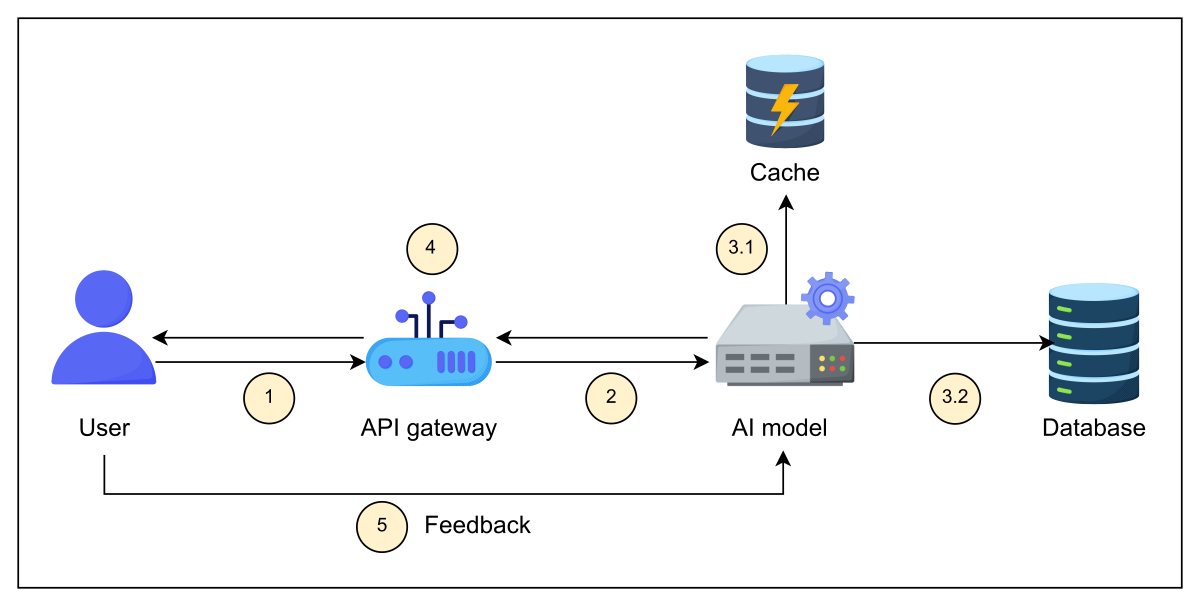
\includegraphics[width=0.5\textwidth]{Images/chapter_41/section_4771659539939328/6016704792363008.png}
 \caption{The high-level design of the ChatGPT system}
\end{figure}

The workflow for the high-level design is provided below:

\begin{enumerate}
\item
\protect\phantomsection\label{8mzZKsWPmt-KID0i4ItoU}
The user submits a text prompt through the interface or an API.
\item
\protect\phantomsection\label{Sak06VfIkPWCQn8XOJVdB}
The API gateway receives the request, handles authentication, rate limiting, and session management, and then forwards the prompt to the model server for processing.
\item
\protect\phantomsection\label{XdnYQP84keYArQY-qheYY}
The AI model processes the provided prompt and uses the conversation history to generate a response. These responses are stored in the cache to quickly retrieve repeated or similar requests and saved in the database for logging, analytics, or future reference.
\item
\protect\phantomsection\label{KDaxn3jT7v4PSz4UbkMMA}
The final response is sent back to the user via the API gateway.
\item
\protect\phantomsection\label{-V-720nrq0v6LmbPf_GEv}
User feedback is collected and stored to help improve system performance and guide future model updates or retraining.
\end{enumerate}
\\
Did you know that every piece of feedback you provide helps ChatGPT grow smarter? It is used to fine-tune the system by enhancing its ability to generate more accurate and natural responses.
\\
Curious about how this process works? Dive deeper into ``\href{https://www.educative.io/courses/generative-ai-system-design/deploying-the-system-design-of-a-text-to-text-generation-system}{System Design of a Text-to-Text Generation System}.''

\begin{quote}
\textbf{Quiz:}
\textbf{Question 1:} Is a typical cache (like LRU or TTL-based) sufficient for storing

AI-generated responses?
\textbf{Answer:} While traditional caching strategies such as LRU or TTL are effective for static or frequently accessed web content, they are often inadequate for AI-generated responses, which are highly contextual and dependent on nuanced input factors such as prompt wording, user history, and personalization. To address this, ChatGPT-like systems benefit from a semantic cache that stores not only the response but also a vector embedding of the input prompt that captures its meaning. When a new prompt is received, the system can retrieve previous responses whose embeddings are semantically similar using a vector-based cache powered by approximate nearest neighbor (ANN) search. This enables the reuse of responses based on meaning rather than exact text matches. So hybrid approach proves to be more effective in maintaining performance,

relevance, and scalability.
\end{quote}

With the high-level architecture in place, let's explore the detailed design:

\subsection{Detailed design of ChatGPT}\label{2uyoYloq392NOnVAQpxw2}
\\
The high-level design gives us a broad overview, but the real magic lies in the detailed design, where we break down the technical intricacies of ChatGPT's architecture. Let 's explore each key component in depth before diving into how they come together in the system's workflow:

\subsubsection{Components in the detailed design of ChatGPT}\label{Dp-oV8vBCIZ8w3xOZRst2}
\\
Each component plays a crucial role in making ChatGPT function seamlessly. The user's requests are routed through the API gateway to a load balancer that distributes traffic efficiently across application servers. The detailed design of the ChatGPT system involves the following components:

\begin{itemize}
\item
\protect\phantomsection\label{ZK0otXLDeQr-cm9sN2UUs}
\textbf{Pre-processing (NLU service):} This service processes user input by extracting meaning, intent, and key entities while converting text into numerical embeddings(An embedding is a vector that captures the meaning of text by placing semantically similar inputs close together in a numerical space.). These embeddings capture semantic relationships, enabling the model to generate contextually relevant responses.
\item
\protect\phantomsection\label{Z4PvTtfFUfn89Z_4amKzx}
\textbf{Model server:} This is the core processing unit that hosts the AI models. It generates responses based on user queries.
\item
\protect\phantomsection\label{6AWcUc2qsht4YolKCgFEI}
\textbf{Vector database:} It stores vector embeddings of past conversations and relevant external knowledge. It allows the system to retrieve semantically similar content, thereby facilitating context-aware responses.
\item
\protect\phantomsection\label{3XTsOqUAZtGOnFe0kGnsh}
\textbf{Redis (caching layer):} It temporarily stores recent conversation history to avoid repeated database lookups and ultimately improves response time.
\end{itemize}

\begin{figure}[htbp]
 \centering
 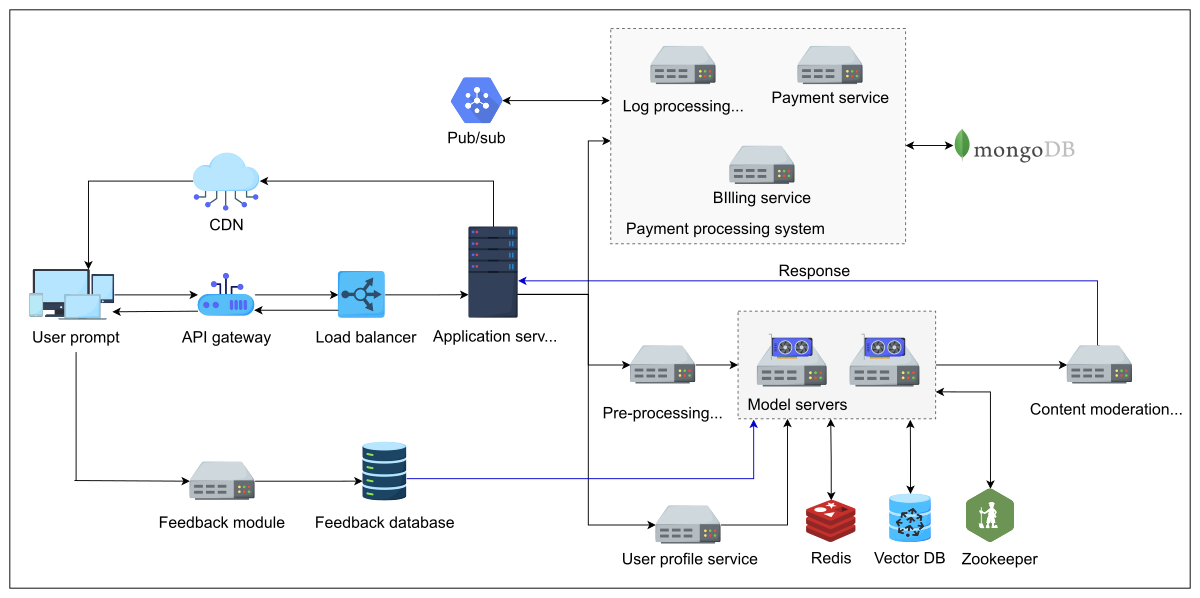
\includegraphics[width=0.5\textwidth]{Images/chapter_41/section_4771659539939328/6207721986457600.png}
 \caption{Detailed design of a text-to-text generation system like ChatGPT}
\end{figure}

\begin{itemize}
\item
\protect\phantomsection\label{YP6oETmdWhP3JbdJ-82IS}
\textbf{Content moderation system:} This system scans responses for policy violations and inappropriate or sensitive content before delivering them to the user.
\item
\protect\phantomsection\label{fMI0N8uf-Fppm7VUviLQB}
\textbf{User profile service:} This service manages authentication while tracking user sessions and storing preferences. It ensures a personalized experience based on past interactions.
\item
\protect\phantomsection\label{IWn8JW8aJl1RFdb4WVduO}
\textbf{Zookeeper (orchestrator):} It coordinates model server management by tracking active instances, distributing workloads, and handling failovers. It ensures smooth service discovery and configuration updates for real-time request handling.
\item
\protect\phantomsection\label{Jhg19x2Qrrd-DodniITj6}
\textbf{Pub/sub:} It manages asynchronous communication between various backend services, including the payment system, by ensuring that events like billing updates, logins, or request failures propagate without blocking API calls.
\item
\protect\phantomsection\label{tqobCarfY9CeGWm1UyX7D}
\textbf{Payment processing system:} This system handles payment-related tasks such as logging transactions, generating bills, and processing payments, all coordinated through a pub/sub-system for seamless communication.
\item
\protect\phantomsection\label{XGzhlxZrfPtnH5t0i0TmC}
\textbf{MongoDB (user database):} It stores structured data like session metadata, payment data, and billing history. This choice is driven by MongoDB\textquotesingle s support for flexible data models, horizontal scalability, and high availability.
\end{itemize}

\begin{quote}
\textbf{Quiz:}
\textbf{Question 1:} How does the payment system determine how much to charge a user for a request in a system like ChatGPT, especially when billing is based on token usage or premium features?
\textbf{Answer:} The payment system calculates charges based on usage logs/data, which track details like the number of tokens used, the complexity of the request, and any premium features accessed. After processing the request, the billing service computes the appropriate cost based on factors like token count or other pricing metrics. This information is then sent to the payment system for user approval to ensure that the user is fully informed and consents to the charge before finalizing the transaction.
\end{quote}

Now, let's walk through the step-by-step journey of processing a user's prompt.

\subsubsection{Workflow of the ChatGPT system}\label{Os0AYFBmmeodEi7wY7Yjl}
\\
When a user enters a prompt through a web or mobile interface, the request first reaches the API gateway, which manages authentication, authorization, and rate limiting. From there, a load balancer distributes the request across multiple application servers to ensure efficient handling.
\\
Before reaching the model, the prompt passes through the preprocessing NLU service. If the user has interacted before, a user profile service retrieves relevant historical data to personalize the response. Once preprocessed, the request is sent to the model servers, where the large language model (LLM) generates a response. When additional context is required, the system queries the vector database to retrieve semantically relevant information from past interactions.
\\
Before the response is returned, it passes through the content moderation system to filter out harmful or inappropriate content. Zookeeper coordinates the model servers by managing configuration, leader election, and health monitoring during scaling and failover.
\\
If the request involves a paid feature, the payment processing system logs the transaction and updates records in MongoDB. Meanwhile , a CDN ensures static assets, such as UI elements, load quickly, but generated responses from the model are handled separately.
\\
Finally, the response is sent back to the user. If the user provides feedback, it is collected via the feedback module and stored in the feedback database. Structured feedback (like ratings or thumbs up/down) goes into a relational database (e.g., PostgreSQL or MySQL). In contrast, unstructured feedback (such as comments or session metadata) is stored in a document database like MongoDB. This data helps improve the system over time through analysis and model updates.
\\
Why is content moderation placed after response generation rather than before?
\\
Use the AI assessment widget below to submit your solution and get an interactive response.

\textbf{Question:}

Content moderation

\textbf{Reference Answer:}

Because moderation must evaluate the actual generated output to filter harmful or inappropriate content, which cannot be fully predicted before generation.

We've explored the detailed design and workflow of the ChatGPT system. Now it's time for the real test! Let's assess how effectively it meets the key requirements and performs under real-world conditions.

\subsubsection{Achieving requirements}\label{Gjuj806_wvZfCyRWOlPRC}
\\
Let's see how our proposed ChatGPT system fulfills the functional and non-functional requirements that we identified in the previous lesson:
\\
\paragraph{Achieving functional requirements}\label{_OKbOlzbzHj-034A8PC2U}
\\
A thoughtfully engineered system should primarily ensure that it meets its intended functionality. The table below illustrates how our design addresses the functional requirements to effectively fulfill the system's overall objectives.

\begin{table}[htbp]
\centering
\small
\adjustbox{max width=\textwidth}{
\begin{tabular}{|p{0.273\textwidth}|p{0.677\textwidth}|}
\hline
\textbf{Functional Requirements} & \textbf{Techniques} \\
\hline
\hline
Dialogue management & \begin{itemize} \tightlist \item The pre-processing NLU service interprets user input.~ \item The model server generates context-aware responses.~ \item User profile service maintains the session context. \end{itemize} \\
\hline
Natural language understanding & \begin{itemize} \tightlist \item The pre-processing NLU service extracts intent and entities~and understands user input. \item Vector DB enables semantic retrieval.~ \item Redis caches recent context for fast access. \end{itemize} \\
\hline
Personalization & \begin{itemize} \tightlist \item User profile stores preferences and history.~ \item Model server uses this data for tailored responses. \end{itemize} \\
\hline
Feedback & \begin{itemize} \tightlist \item Feedback module logs user ratings and comments, which are used to refine the system through offline training and model improvements. \end{itemize} \\
\hline
\end{tabular}
}
\end{table}

\paragraph{Achieving non-functional requirements}\label{iPEwcXSpqkOfweKRnzmjv}
\\
An effective system must not only operate correctly but also satisfy its non-functional requirements. These requirements define the system's performance, reliability, and scalability in real-world environments. The table below highlights how our design tackles the non-functional requirements:

\begin{table}[htbp]
\centering
\small
\adjustbox{max width=\textwidth}{
\begin{tabular}{|p{0.307\textwidth}|p{0.643\textwidth}|}
\hline
\textbf{Non-functional Requirement} & \textbf{Techniques} \\
\hline
\hline
\hfill\break Scalability & \begin{itemize} \tightlist \item The load balancers~distribute traffic across multiple servers.~ \item Model servers and vector database~scale horizontally as demand grows.~ \item Redis caching~reduces redundant processing. \end{itemize} \\
\hline
\hfill\break \hfill\break Reliability and availability & \begin{itemize} \tightlist \item Zookeeper~coordinates distributed components for fault tolerance.~ \item Redundant model servers and databases~ensure continued operation in case of failures.~ \item Pub-sub enables decoupled communication for real-time updates and seamless failure recovery. \end{itemize} \\
\hline
\hfill\break Low latency & \begin{itemize} \tightlist \item Redis caching accelerates responses for frequently queried data. \item Vector database~efficiently retrieves contextual information, reducing unnecessary recomputation. \item CDN reduces latency by caching and serving static content closer to users. \end{itemize} \\
\hline
\hfill\break \hfill\break Security and privacy & \begin{itemize} \tightlist \item API gateway~enforces authentication, authorization, and rate limiting.~ \item Payment processing system~ensures secure financial transactions. \item End-to-end encryption~secures requests and responses from interception. \item MongoDB stores user data with encryption and access control. \end{itemize} \\
\hline
\end{tabular}
}
\end{table}

\subsection{Conclusion}\label{3y0zGOifMPf7VYecYjlTG}
\\
In this chapter, we designed a ChatGPT-like system, covering everything from high-level architecture to detailed workflows. We saw how it ensures scalability, reliability, and security while delivering real-time, context-aware responses through components like caching, content moderation, and distributed model hosting.
\\
But this is only the beginning.

\begin{itemize}
\item
\protect\phantomsection\label{MqIzJ4-Msvgkhgatlu0AE}
While we discussed the context-awareness module, how is that actually created and integrated into the system?
\item
\protect\phantomsection\label{FlK8aCEb6OjS7XNL6yD-j}
How is user feedback incorporated in the subsequent responses generated by the GenAI System?
\end{itemize}
\\
To develop a deeper understanding of the questions above, explore~\href{https://www.educative.io/courses//generative-ai-system-design}{Grokking the Generative AI System Design}.
\\
Looking ahead, advances in LLMs, RAG(Retrieval-augmented generation), and efficient inference will enhance performance, while trends such as multimodal AI and on-device inference may make ChatGPT-like systems more responsive and personalized.

% End of section content